\mysection{Henchmen}{gear-henchmen}

\mysubsection{Loyalty}{gear-henchmen-loyalty-checks}

Whether linkboys or meatshields, all henchmen have \mybold{Loyalty} to you, similar to \mylink{Monster's Morale}{monster-morale}.  When you make a Loyalty try for your henchmen, roll a 2d6. If the result is greater than or equal to the henchman's Loyalty, they'll refuse to do what you're trying to coax them into doing.  If you wish, you can roll your \PRE and add it to the Loyalty try, but a) you have to do it before you roll 2d6; b) it only counts for that specific Loyalty check;  and c) if you roll a Failure (a 1 or a 2), the henchman automatically refuses, and their Loyalty goes down by 1.

    Asking a hireling to take more risks than the rest of the party causes them to lose 1 Loyalty, regardless of whether or not they accept or refuse. Good treatment can make their Loyalty go up (to a maximum of 11).  Poor treatment obviously can drop it.  Raising or lowering your henchman's loyalty is at the Arbiter's discretion.


    If a henchmen ever hits 2 Loyalty, they'll try to escape as soon as possible.  Maybe with your stuff.  Maybe they'll try to kill you, too.

\begin{center}
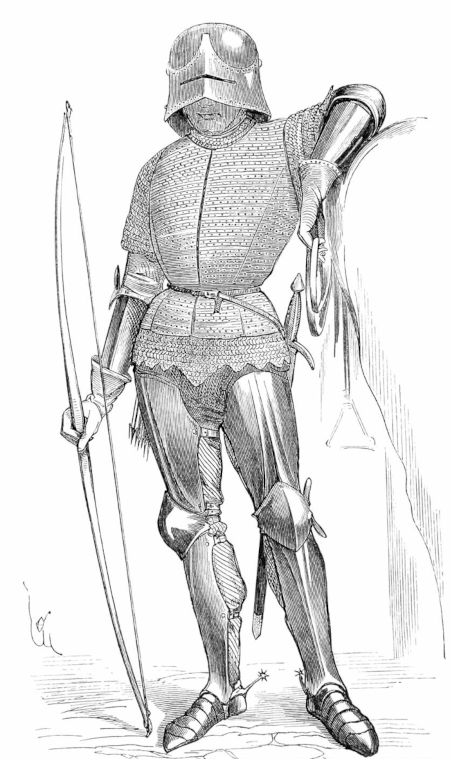
\includegraphics[scale=.3]{gear/Archer}
\end{center}

\cbreak

    \mysubsection{Hirelings}{gear-hirelings}

\callout {\footnotesize{
    Hirelings are non-combatant workers, aides, etc. you can hire for a set rate (usually 5 coins a day) plus food (including providing Provisions during a \mylink{Bivouac}{combat-resting-bivouac}). If a fight breaks out, they run for cover - if they're attacked (like running into an ambush or targeted by a creature) they are immediately killed at the Arbiter's discretion. They'll refuse to do anything overtly risky, but can be coaxed into doing something with minor risk with a Loyalty try.  Overtly risky tasks might be being the first one down a hallway, or pulling an unmarked lever. Moderately risky tasks might standing watch in the hall while the party is in a room.

\myskip

    \mybold{Hirelings have a starting Loyalty of 3.}
}}



    \myhighlight{Cook}{gear-hirelings-cook}

    Good to have on \mylink{long journeys}{movement-travel}.  If you ever need to roll your Party Provisions, the Cook is Skilled (d12+2) in \mylink{Skill: Travel}{skill-travel}, but only when it comes to food.

    \myhighlight{Guides}{gear-hirelings-guides}

    Folks who know how to get to somewhere specific. Useful if you're \mylink{Traveling}{movement-travel} off the beaten track. Guides are Skilled (d12+2) in \mylink{Skill: Travel}{skill-travel}, but only to a specific location.


    \myhighlight{Linkboys}{gear-hirelings-linkboys}

    Linkboys hold torches so you don't have to (torches not included). They can carry up to 6 \mylink{Burden}{gear-burden} of gear.

    \myhighlight{Porters}{gear-hirelings-porters}

    Beefy numbskulls hired to carry your stuff. They can carry 12 \mylink{Burden}{gear-burden} of gear.


    \mysubsection{Mercenaries}{gear-mercenaries}

\callout {\footnotesize {
    More potent than your typical Hireling, mercenaries will work for a half share or 10 coins a day (whatever is highest) plus food (including providing Provisions during a \mylink{Bivouac}{combat-resting-bivouac}).  A mercenary will try to stay as close to the person who hired them as possible.  They stand in the background but don't generally shirk from combat. They'll have to try their Loyalty if they're asked to do something overtly risky.  In combat, they'll need to check Loyalty a) when the first Adventurer starts \mylink{Dying}{combat-dying}; b) when half the Adventurers are incapacitated; and c) if the person they're attached to becomes incapacitated.

\myskip

    \mybold{Mercenaries have a starting Loyalty of 6.}
}}


    \myhighlight{Bard}{gear-mercenary-bard}

    Singers and storytellers, Bards are able to perform the \mylink{Vulgate of Charms}{vulgate-charms}. During a \mylink{Breather}{combat-resting-breather}, roll a 2d6 - the Bard is able to restore \SUM \mylink{Grit}{adventurer-flesh-grit} during a Breather, distributed any way the Band wishes. Bards are Skilled (d12+2) in \mylink{Skill: Lore}{skill-lore}, and will keep a record of your exploits to regale people with.  If a fight breaks out, they run for cover - if they're attacked (like running into an ambush or targeted by a creature) they are immediately killed at the Arbiter's discretion.  They refuse to share the spotlight with other bards.

    \myhighlight{Meatshield}{gear-mercenary-meatshield}

    In Combat, a Meatshield can (a) grant you +1 to your Attack or Guard \RO; (b) grant you +1 to damage; or (c) take any physical damage for you.  You have to specify what each Meatshield is doing at the top of each Moment i.e. "1 is giving me +1 damage and I'm keeping one back to take damage in case things go south." but they don't take a combat turn themselves.  Any physical damage you would take you can put onto the Meatshield instead.  Meatshields have 4 Flesh and 4 Grit, but you can give them Armor if you like. You can employ up to 2 Meatshields (any more than that starts to look like an army).


    \myhighlight{Mechanic}{gear-mercenary-mechanic}

    A Mechanic can be coaxed into picking locks, removing traps, and scouting rooms.  They are Skilled (d12+2) in \mylink{Skill: Tinkering}{skill-tinkering}.  They give you a +1 to your Attack and Guard \RO, but they don't take a combat turn themselves.  Any physical damage you would take you can put onto the Mechanic instead.  They have 4 Flesh, 0 Grit, and can't wear any Armor. They refuse to work with other Mechanics in the party.

    \myhighlight{Vicar}{gear-mercenary-vicars}

    Vicars are holy people of a sort, able to perform the \mylink{Vulgate of Sacraments}{vulgate-sacraments} on behalf of the Band. Vicars take no Combat Actions, but they have a \mylink{Grace Die}{vulgate-sacraments} with which to perform any of the Sacraments. Not being fighting types, they always take a turn \myital{after} the Monsters take their turn. They have 4 Flesh, and can wear Armor - but assume any attacks that hit them succeed automatically. Employing more than one Vicar of a different religion can result in ... complications.

\myimage{gear/Hireling}
